\documentclass[11pt]{standalone}
\usepackage{amssymb}
\usepackage{amsmath}
\usepackage[no-math]{fontspec}
\usepackage{unicode-math}
\usepackage{libertinus}
\usepackage{pgf,xcolor}
\usepackage{tikz}
\usetikzlibrary{arrows.meta, backgrounds}
\usepackage{pgfplots}
\pgfplotsset{compat=newest}

\definecolor{my_darkgray}{HTML}{484949}
\definecolor{my_lightgray}{HTML}{F3F4F4}
\definecolor{my_darkblue}{HTML}{005A94}
\definecolor{my_lightblue}{HTML}{CCDEE9}
\definecolor{my_yellow}{HTML}{FFEC7F}
\definecolor{my_red}{HTML}{E60000}
\definecolor{my_orange}{HTML}{E87846}

\begin{document}
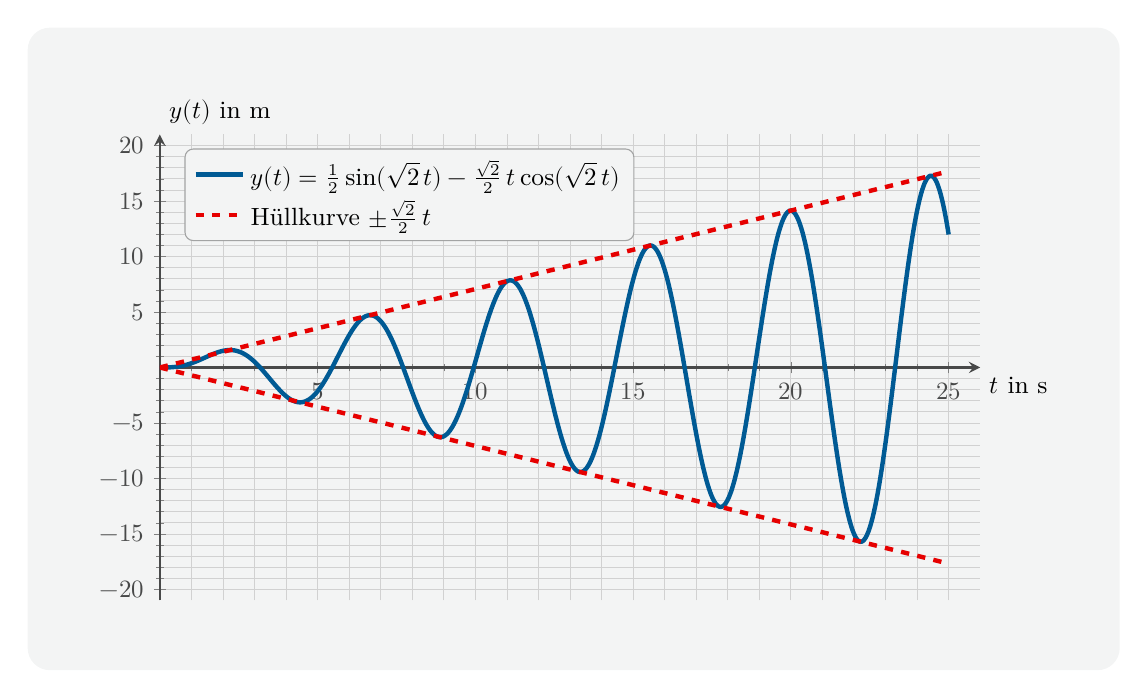
\begin{tikzpicture}[
    show background rectangle,
    background rectangle/.style={fill=my_lightgray, rounded corners=8pt},
    inner frame sep=0.8cm
]
\begin{axis}[
    % axis equal weggelassen: t in s und y(t) in m haben sehr unterschiedliche
    % Wertebereiche; gleiche Skalierung würde den Graphen unleserlich machen.
    axis lines=center,
    xlabel={$t$ in s},
    ylabel={$y(t)$ in m},
    xlabel style={at={(ticklabel* cs:1.0)}, anchor=north west, font=\small},
    ylabel style={at={(ticklabel* cs:1.0)}, anchor=south west, font=\small},
    grid=both,
    grid style={line width=0.3pt, draw=my_darkgray!25},
    axis line style={thick, draw=my_darkgray},
    width=12cm,
    height=7.5cm,
    xmin=0, xmax=26,
    ymin=-21, ymax=21,
    xtick={0, 5, 10, 15, 20, 25},
    ytick={-20, -15, -10, -5, 0, 5, 10, 15, 20},
    tick label style={font=\small, color=my_darkgray},
    minor tick num=4,
    samples=600,
    legend pos=north west,
    legend style={
        font=\small,
        fill=my_lightgray,
        draw=my_darkgray!50,
        rounded corners=3pt
    },
    legend cell align=left,
]

%% --- Vollständige Lösung im Resonanzfall Ω = ω₀ = √2 ---
%% y(t) = (1/2)·sin(√2·t) − (√2/2)·t·cos(√2·t)
%% Trig-Argumente in deg() konvertieren, da pgfplots Grad erwartet.
\addplot[draw=my_darkblue, ultra thick, domain=0:25]
    {0.5 * sin(deg(sqrt(2) * x))
     - (sqrt(2) / 2) * x * cos(deg(sqrt(2) * x))};
\addlegendentry{%
    $y(t)=\tfrac{1}{2}\sin(\sqrt{2}\,t)
          -\tfrac{\sqrt{2}}{2}\,t\cos(\sqrt{2}\,t)$}

%% --- Obere Hüllkurve +( √2/2 )·t ---
\addplot[draw=my_red, ultra thick, dashed, domain=0:25]
    {(sqrt(2) / 2) * x};
\addlegendentry{Hüllkurve $\pm\tfrac{\sqrt{2}}{2}\,t$}

%% --- Untere Hüllkurve −( √2/2 )·t  (kein eigener Legendeneintrag) ---
\addplot[draw=my_red, ultra thick, dashed, domain=0:25, forget plot]
    {-(sqrt(2) / 2) * x};

\end{axis}
\end{tikzpicture}
\end{document}
